\documentclass[a4paper,12pt]{article}

\usepackage{graphicx}
\usepackage{amsmath}
\usepackage{float}

\begin{document}

\noindent
\begin{minipage}[t]{0.2\textwidth}

\includegraphics[width=2.5cm]{iiitb_logo.png}
\end{minipage}
\hfill
\begin{minipage}[t]{0.7\textwidth}
\raggedleft
{\Large \textbf{Pavithra Kune}}

COMETFWC069
\end{minipage}

\vspace{1cm}

\begin{center}
{\Large \textbf{GATE QUESTION Q36 - FSM IMPLEMENTATION}}
\end{center}

\hrule

\vspace{0.5cm}

\begin{figure}[H]
\centering
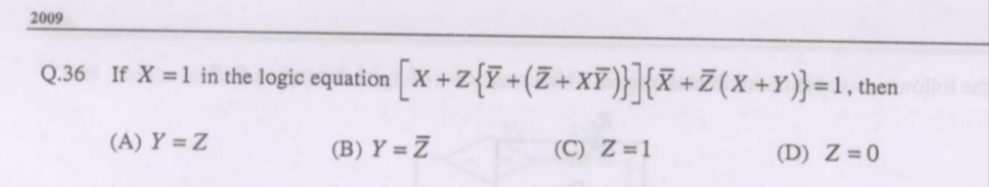
\includegraphics[width=0.8\textwidth]{question.png}
\caption{GATE Question Q36}
\end{figure}

\tableofcontents

\newpage

\section{Components}

Breadboard

Arduino Uno

IC 7474

IC 7447

Seven Segment Display

Jumper Wires

\section{Finite State Machine}

A Finite State Machine (FSM) is a sequential circuit that changes from one state to another based on the clock input.

The present state is represented by

\[
W,X,Y,Z
\]

and the next state is represented by

\[
A,B,C,D
\]

In this implementation, the FSM behaves as a decade counter. The state increments by one on every clock pulse and resets to zero after state 9.

\section{Hardware Connections}

Arduino Pin D6 is connected to W.

Arduino Pin D7 is connected to X.

Arduino Pin D8 is connected to Y.

Arduino Pin D9 is connected to Z.

Arduino Pin D2 is connected to A of IC 7447.

Arduino Pin D3 is connected to B of IC 7447.

Arduino Pin D4 is connected to C of IC 7447.

Arduino Pin D5 is connected to D of IC 7447.

Arduino Pin D13 is connected to Clock.

\section{Software Implementation}

\begin{verbatim}
#include <Arduino.h>

int W,X,Y,Z;
int D,C,B,A;

void disp_fsm(int D,int C,int B,int A)
{
  digitalWrite(2,A);
  digitalWrite(3,B);
  digitalWrite(4,C);
  digitalWrite(5,D);
}

void setup()
{
  pinMode(2,OUTPUT);
  pinMode(3,OUTPUT);
  pinMode(4,OUTPUT);
  pinMode(5,OUTPUT);

  pinMode(6,INPUT);
  pinMode(7,INPUT);
  pinMode(8,INPUT);
  pinMode(9,INPUT);

  pinMode(13,OUTPUT);
}

void loop()
{
  digitalWrite(13,HIGH);
  delay(10);
  digitalWrite(13,LOW);

  W = digitalRead(6);
  X = digitalRead(7);
  Y = digitalRead(8);
  Z = digitalRead(9);

  int state = (Z<<3)|(Y<<2)|(X<<1)|W;
  int next = (state >= 9) ? 0 : state + 1;

  A = (next>>0)&1;
  B = (next>>1)&1;
  C = (next>>2)&1;
  D = (next>>3)&1;

  disp_fsm(D,C,B,A);

  delay(1000);
}
\end{verbatim}

\section{Output}

\begin{figure}[H]
\centering
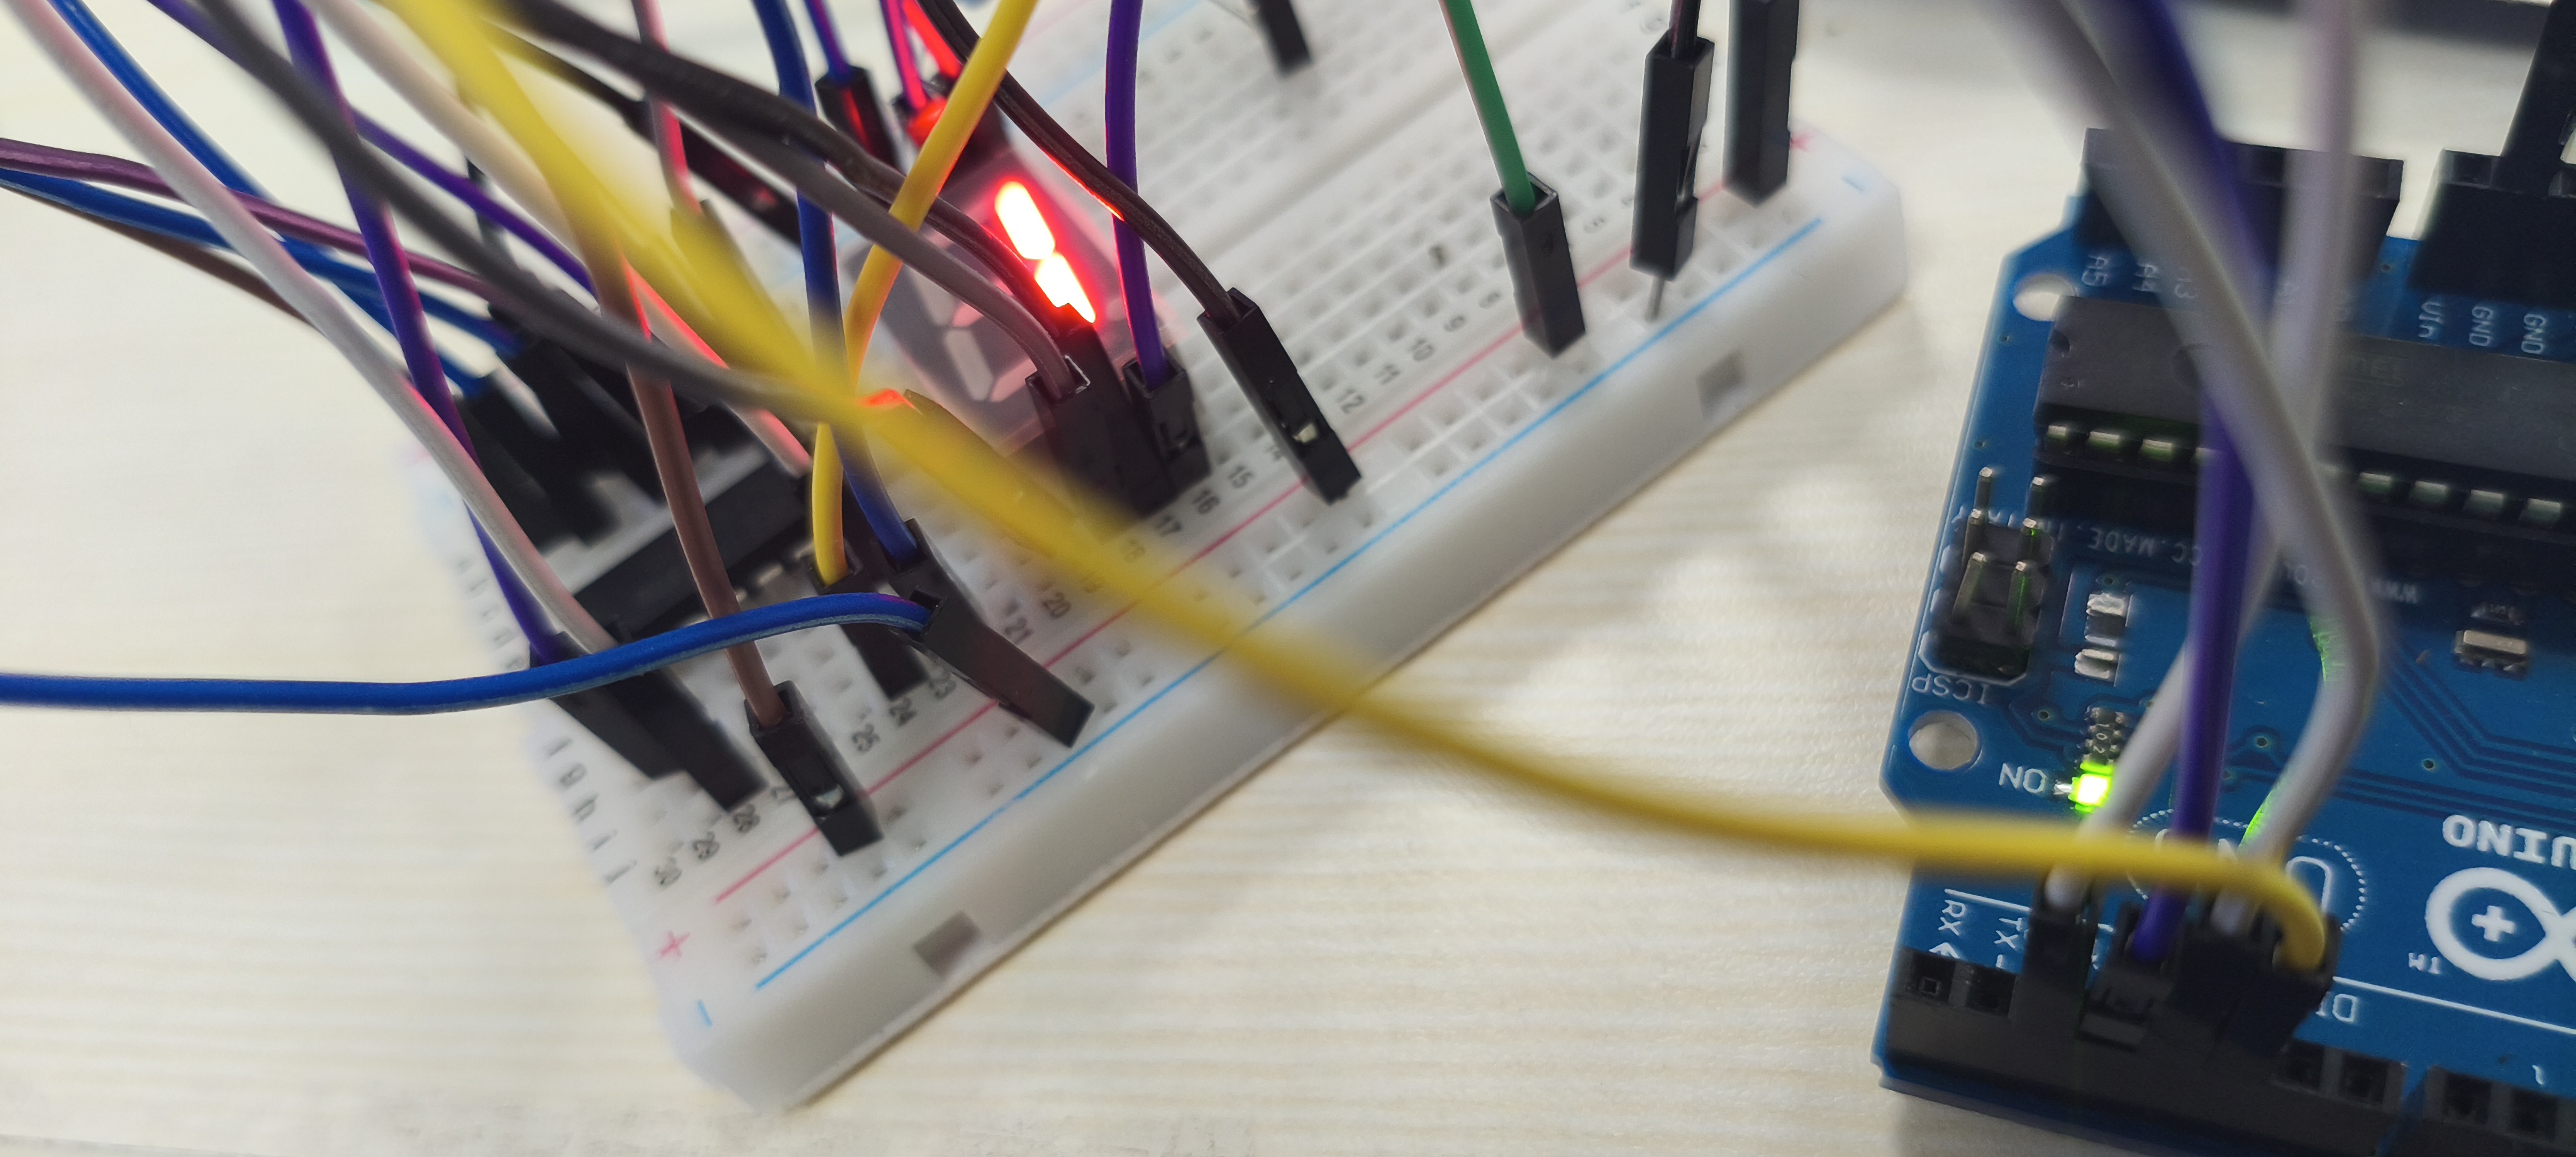
\includegraphics[width=0.45\textwidth]{output1.jpg}
\caption{FSM Output}
\end{figure}

\section{Result}

The Finite State Machine for a decade counter was implemented using Arduino Uno, IC 7474, IC 7447 and a seven segment display.

The FSM increments its state on every clock pulse and displays the corresponding decimal digit on the seven segment display.

\end{document}
